%# -*- coding: utf-8-unix -*-
%%==================================================
%% chapter01.tex for SJTU Master Thesis
%%==================================================

%\bibliographystyle{sjtu2}%[此处用于每章都生产参考文献]
\chapter{AKI——实际密钥信息}
\label{chap:AKI}
轮函数的完全扩散性(completeness,即任意一个输出比特都依赖于所有的输入比特)是衡量一个轮函数扩散程度的重要标准。
对于非完全扩散的轮函数,考察其扩散的程度就变得极为重要。
为了精确考察密钥编排方案的弱点导致实际攻击的一般规律,黄佳琳博士在其博士毕业论文\citen{黄佳琳2014分组密码}中提出了实际密钥信息这一概念,从而考察了一个密钥编排方案在给定轮函数时的强弱程度。
\section{AKI的定义}
黄佳琳博士在\citen{huang2014revisiting}中提出了基于密钥依赖路径的实际密钥信息定义,而实际上实际密钥信息可适用于任何子密钥集合。因此,在本节中,我们扩展了黄佳琳博士对AKI的定义:
\begin{defn}[密钥信息集合(Key Information, KI)]
    给定一个子密钥集合$K$,如果通过密钥编排方案,使用另一个子密钥集合$K_0$可以计算出$K$中的所有比特,则称$K_0$是$K$的一个密钥信息集合。
\end{defn}
\begin{defn}[实际密钥信息(Actual Key Information, AKI)]
    给定一个子密钥集合$K$,其密钥信息集合中最小的集合被成为实际密钥信息集合,实际密钥信息集合的大小即为$K$所包含的实际密钥信息。
\end{defn}
在实际密码攻击方法中,子密钥猜测环节十分常见且重要,例如相关密钥攻击\citen{biham1994new}和中间相遇攻击\citen{diffie1977special}.
在这些攻击中,将子密钥猜测集合替换为其实际密钥信息集合,就可以在不影响猜测的信息的情况下降低需要猜测的比特数量,从而降低攻击的复杂度。
\section{密钥编排方案的密钥信息}
黄佳琳博士在\citen{huang2014revisiting}中提出了使用AKI来分析给定一个轮函数的情况下一个密钥编排方案强弱的方法。
\begin{defn}[计算路径]
    设$O_0$为一个$m$比特的中间状态。根据轮函数我们可以得到一条$O_0$的计算路径:
    $$O_0=f_1(O_1,K_1)=f_1(f_2(O_2,K_2),K_1)=\dots f_1(\dots(f_s(O_s,K_s),K_{s-1}),\dots,K_1),$$
    其中$f_i$依赖于分组密码的结构和第$i$轮的轮函数,而$O_i$, $O_{i-1}$分别为第$i$轮的输入比特集合和输出比特集合,$O_{i-1}$的计算依赖于$O_i$和$K_i$(计算$O_{i-1}$所需要的密钥比特)。
    $O_0\rightarrow O_1\rightarrow O_2\rightarrow\dots\rightarrow O_s$被成为一条计算路径,其中$O_0$和$O_s$分别为该路径的输出和输入。
\end{defn}
为了构造$O_0$的一条计算路径,我们需要从$O_0$开始往前轮寻找所有计算$O_0$所需要的比特,而这些比特加上$O_0$本身则构成了$O_0$的一条计算路径。
而计算$O_{i-1}$所依赖的$K_i$所构成的集合则被定义为:
\begin{defn}[密钥依赖路径]
    一条计算路径上所涉及的所有轮密钥比特所构成的集合称为该计算路径的密钥依赖路径,即$K_1,K_2,\dots,K_s$。
\end{defn}
密钥依赖路径实际上包含了为了计算$O_0$所需要的所有的轮密钥比特。

%一般来说,一个密钥编排方案包含了密钥提取和密钥扩展两个部分。
%\begin{defn}[密钥提取]
%    密钥提取是密钥编排方案中从第$i$轮的密钥寄存器中的子密钥$WK_i$提取出要使用在轮函数中的轮密钥$RK_i$的过程。
%\end{defn}
%\begin{defn}[密钥扩展]
%    密钥提取是密钥编排方案中从第$i$轮的密钥寄存器中的子密钥$WK_i$生成第$i+1$轮的子密钥$WK_{i+1}$的过程。
%\end{defn}
%由于对于一个密钥编排方案来说,改变密钥提取方案本质上只是改变了子密钥$WK_i$中比特的顺序,因此为了将目光着重放在密钥扩展上,
一般来说,密钥编排方案是一个将主密钥扩展成更长的扩展密钥并使用作轮密钥的算法。
为了设计密钥编排方案时的统一性,我们给出一个更一般的密钥编排方案的定义:
\begin{defn}[密钥编排方案]
    一个密钥编排方案算法$g$包含子密钥生成和轮密钥提取两部分。子密钥$WK_i$一般指第$i$轮密钥寄存器中的密钥比特,$WK_i$包含主密钥中的所有信息(故一般$WK_i$长度与主密钥相等),且$WK_{i+1}$可以通过子密钥生成算法由$WK_i$推出;
    轮密钥$RK_i$是子密钥$WK_i$中的一些比特,由轮密钥提取算法从$WK_i$中提取出。
    即密钥编排方案$g$中每轮均有以下操作:
    $$g_i:\begin{cases}
        WK_i=KeyExpand_i(WK_{i-1})\\
        RK_i=KeyExtract_i(WK_i)
    \end{cases}$$
\end{defn}

为了软硬件上实现的高效性,密钥编排方案中每一轮的子密钥生成和密钥提取算法一般是相同的(部分密码的密钥编排方案中会有所不同,如IDEA密码\citen{lai1990proposal}中密钥提取均不相同)。
在本文中,凡是未提前定义的密钥编排方案,其密钥提取方案默认为简单提取,即$RK_i^j=WK_i^j$。
由于密钥依赖路径中包含的是计算$O_0$所需要的轮密钥比特$RK$,因此密钥依赖路径的计算只依赖于轮函数,与密钥编排方案无关,因此给定轮函数的情况下,不同密钥编排方案下同一条密钥依赖路径的实际密钥信息的不同可以用来考察该密钥编排方案在此轮函数情况下的强弱程度。

为了更方便的计算以上两条路径,我们需要量化轮函数和密钥编排方案子密钥生成中输入比特和输出比特的依赖关系。
\begin{defn}[依赖矩阵]
    一个依赖矩阵$M=M_{i,j}\in\mathbb{F}^{n\times n}_2$包含了单轮输入输出比特之间的依赖关系,其中$M_{i,j}=1$表示第$i$个输出比特依赖于第$j$个输入比特,反之$M_{i,j}=0$表示不依赖。\footnote{值得一提的是,加密算法和解密算法所对应的依赖矩阵不一定互为逆矩阵,需要以实际情况推论。}
\end{defn}

接下来,我们给出对于一个加密方案,单轮的AKI的定义:
\begin{defn}[单轮实际密钥信息]
    一个加密方案中,第$i$轮的单轮实际密钥信息$AKI_i$是该轮中间状态$X_i$中所有单个比特对应的密钥依赖路径的实际密钥信息的最小值。
    \label{def:RoundAKI}
\end{defn}
\begin{thm}
    单轮实际密钥信息$AKI_i$随轮数$i$的增加而单调递增(但不一定严格递增)。
\end{thm}
\noindent
\textbf{证明:}对于第$i$轮中间状态上的比特$X_i^j$和它依赖的一个第$i-1$轮上的比特$X_{i-1}^k$,由$X_i^j$得到的计算路径必然包含了由$X_{i-1}^k$得到的计算路径(因为计算$X_{i-1}^k$所需要的比特必然被计算$X_i^j$所需要),因此两者相对应的密钥依赖路径(记作$KDP_i^j$和$KDP_{i-1}^k$)也同样由着前者包含后者的关系($KDP_{i-1}^k\subseteq KDP_i^j$)。
显然,一个子密钥集合的实际密钥信息不可能小于它的一个子集的实际密钥信息,因此$KDP_i^j$的实际密钥信息$AKI_i^j$必然大于等于$KDP_{i-1}^k$的实际密钥信息$AKI_{i-1}^k$。
所以我们有:
$$AKI_i^j\geq AKI_{i-1}^k\geq AKI_{i-1}$$
即第$i$轮上任意一比特对应的密钥依赖路径的实际密钥信息均大于等于第$i-1$轮的单轮实际密钥信息,因此第$i$轮的单轮实际密钥信息也会大于等于第$i-1$轮的单轮实际密钥信息。\qed

单轮实际密钥信息描述了该轮所包含的密钥信息的下界。
一个正常的密钥编排方案应该在某一轮的单轮实际密钥信息达到理论最大值(主密钥长度$n$),否则说明了主密钥没有完全被使用。
对于衡量一个密钥编排方案来说,这是一个重要的指标。
我们会在第\ref{chap:App}、\ref{chap:Design}和\ref{chap:Work}章中多次使用这个定义。
一个理想的密钥编排方案应该在最少的轮数就能达到理论最大值,这是我们设计密钥编排方案的核心思想与目标。在第\ref{chap:Design}章中我们会着重讨论这一点。

\begin{figure}[htbp]
\centering
    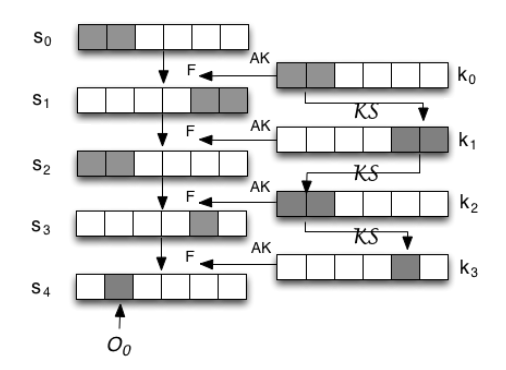
\includegraphics[width=6cm]{ToyCipher}
    \bicaption[fig:toy]{玩具密码}{一个4轮的玩具密码}{ToyCipher}{A 4-round toy cipher}
\end{figure}
\textbf{一个典型的例子\citen{Huang_2014}:}
图\ref{fig:toy}是一个4轮SPN结构的玩具密码,其分组大小和主密钥长度均为6比特,每一个中间状态都直接与相对应的轮密钥进行异或。
其轮函数依赖矩阵为$M_s$,密钥编排方案的依赖矩阵为$M_k$(这里给出了三个不同的编排方案$M_{k1},M_{k2},M_{k3}$)。
$$M_s=\left(
    \begin{array}{cccccc}
        0&0&0&0&0&1\\
        0&0&0&0&1&1\\
        0&0&0&1&0&0\\
        0&0&1&1&0&0\\
        0&1&0&0&0&0\\
        1&1&0&0&0&0
    \end{array}
\right)$$
$$M_k=\left(
    \begin{array}{cccccc}
        0&0&0&0&0&1\\
        0&0&0&0&1&1\\
        0&0&0&1&0&0\\
        0&0&1&1&0&0\\
        0&1&0&0&0&0\\
        1&1&0&0&0&0
    \end{array}
\right)
or\left(
    \begin{array}{cccccc}
        1&0&0&0&0&0\\
        0&1&0&1&0&0\\
        0&0&0&0&1&0\\
        1&0&0&0&0&1\\
        0&0&1&0&0&0\\
        0&0&0&1&0&1
    \end{array}
\right)
or\left(
    \begin{array}{cccccc}
        1&0&1&0&0&0\\
        0&0&0&1&0&0\\
        0&1&0&0&1&0\\
        1&0&0&0&0&0\\
        0&0&1&0&0&1\\
        0&0&0&0&1&0
    \end{array}
\right)$$
令$O_0$只保含了第4轮的第2比特(记为$X_4^1$),我们可以根据轮函数依赖矩阵$M_s$计算出其计算路径:$\{X_0^0,X_0^1\}\rightarrow \{X_1^4,X_1^5\}\rightarrow \{X_2^0,X_2^1\}\rightarrow \{X_3^4\}\rightarrow \{X_4^1\}$。
相对应的,其密钥依赖路径为$\{WK_0^0,WK_0^1\}\rightarrow \{WK_1^4,WK_1^5\}\rightarrow \{WK_2^0,WK_2^1\}\rightarrow \{WK_3^4\}$。
注意到密钥依赖路径中包含了7比特的子密钥,但考虑到主密钥长度只有6比特,因此该密钥依赖路径的所包含的实际密钥信息理论上不可能超过6比特。

在三个密钥编排方案中,密钥编排方案$M_{k1}$由于其与轮函数的依赖关系完全一样,导致密钥依赖路径上各轮比特之间存在与轮函数完全一致的依赖关系,则只用密钥依赖路径在主密钥上的比特就可以推出整条密钥依赖路径。
因此,$\{WK_0^0,WK_0^1\}$就是该密钥依赖路径的一个实际密钥信息集合,AKI仅为2,存在着严重的密钥信息泄露。

而相对的,密钥编排方案$M_{k2}$和$M_{k3}$就表现更好。在编排方案$M_{k2}$下,该密钥依赖路径的AKI为5(其中一个可能的实际密钥信息集合为$\{WK_0^0,WK_0^1,WK_0^2,WK_0^3,WK_0^5\}$),而$M_{k3}$更让AKI达到了理论最大值6。
值得一提的是,$M_{k3}$能够使所有第4轮比特的密钥依赖路径的AKI都达到理论最大值6,即$M_{k3}$使得该玩具密码在经过4轮加密之后不存在任何密钥信息泄露。

因此,AKI不仅在攻击中能够降低某些攻击的复杂度,并且一个密钥编排方案的AKI值也是在某种程度上衡量该方案在其轮函数下的强弱程度的重要参数,而后者中的弱编排方案将会导致该密码函数更容易受到前者的影响,降低攻击该函数的复杂度。
同时,由于给定轮函数后不同的编排方案拥有不同的AKI值,使得AKI成为了设计与优化密钥编排方案的重要指标。
